\documentclass[11pt]{article}

\usepackage{wrapfig}
\usepackage{amsmath}
\usepackage[letterpaper,margin=0.7in]{geometry}
\usepackage{tikz}
\usetikzlibrary{calc}
\usepackage{natbib}
\usepackage{linguex}
\usepackage{url}
\bibliographystyle{apalike}

\title{\vspace{-1.5cm}\large \bf \emph{Roses and flowers}: an informativeness implicature in
  probabilistic pragmatics\vspace{-2cm}}
\date{}
%\author{Roger Levy, Leon Bergen, and Noah Goodman}



\renewcommand{\baselinestretch}{0.97}
\begin{document}

\maketitle

\noindent
% One of the outstanding achievements of linguistic pragmatics as a
% field has been the ability to account for a superficially disparate
% collection of inferential patterns through a small set of
% conversational principles.  Beginning with
% \citet{grice:1957,grice:1975}, considerable effort has gone into both
% refining the characterization of these principles and rooting them in
% deeper principles of reasoning under the assumption of cooperation
% \citep[inter alia]{horn:1984,sperber-wilson:1986,levinson:2000}.  
In the half-century since the introduction of Grice's maxims
(\citeyear{grice:1957,grice:1975}), considerable effort has gone
into refining them into a smaller set of generalizations rooted in
deeper principles of cooperative communication \citep[inter
alia]{horn:1984,sperber-wilson:1986,levinson:2000}. One particularly
fruitful result of these efforts has been the identification of a
tension between so-called ``quantity'' implicature, in which
utterances are interpreted as being no stronger than the lower bound
allowed by their literal semantics, as in \ref{ex:quantity-implicature}, and
``informativeness'' implicature, in which utterances are interpreted
as strengthened to a prototypical case, as in
\ref{ex:informativeness-implicature}
\citep{atlas-levinson:1981,horn:1984}:

\ex. \label{ex:quantity-implicature}
\a. Pat has three children$\rightarrow$Pat has exactly three children
\b. I slept in a car yesterday$\rightarrow$The car was not mine 

\ex. I broke a finger yesterday$\rightarrow$The finger was mine \label{ex:informativeness-implicature}

A Bayesian approach to linguistic
interpretation offers the promise that this tension may be a consequence of
 formalizing pragmatic inference as probabilistic reasoning:
 complex interactions are predicted from recursive reasoning involving alternative utterances, shared
beliefs about common communicative goals, prior information about
world state, and utterance costs.  Here we discuss the challenges
posed to a Bayesian pragmatics account by a (to our knowledge,
previously unobserved) pattern of informativeness implicature: when
the conjunction of a superordinate category $X$ with a subordinate
member $x$ of that category, \emph{$x$ and $X$}, receives a
strengthened interpretation equivalent to \emph{$x$ and other $X$}, as
in \ref{ex:roses-and-flowers-example} below:

\ex. We sell roses and flowers for Mother's
Day.\footnote{\url{http://e-clubhouse.org/sites/townofsheboyganwi/}} \label{ex:roses-and-flowers-example}

Corpus analysis shows that English has many such common alternations,
such as \emph{tulips and (other) flowers}, \emph{beef and (other)
  meat}, \emph{horse and (other) animals}, \emph{physicists and (other)
  scientists}, and more.  Longitudinal data show that this is an
historically stable pattern: to take one example, \emph{roses and
  flowers} and \emph{roses and other flowers} have coexisted with
roughly similar relative frequencies since 1800.  An experimental
investigation shows that omitting \emph{other} has no discernible
effect on the referential interpretation of the phrase---naive native
speakers have the same beliefs about how many types of flowers are
being talked about regardless of whether \emph{roses and flowers} or
\emph{roses and other flowers} is used.

The challenge for a formal analysis is thus to show how \emph{roses
  and flowers} can come to be interpreted as meaning the same thing as
\emph{roses and other flowers}.  The immediate challenge for a
strongly neo-Gricean account is that if literal semantics have a
chance to be computed globally, we are stuck with a truth-conditional
meaning for utterances involving \emph{roses and flowers} that is the
same as for utterances involving \emph{roses} alone: for example, the
literal meaning of \ref{ex:roses-example} is the same as that
of~\ref{ex:roses-and-flowers-example}:

\ex. We sell roses for Mother's Day. \label{ex:roses-example}

\noindent
The pragmatic strengthening of~\ref{ex:roses-and-flowers-example}  to mean \emph{roses and other 
  flowers} must thus be an instance of the ``division of pragmatic
labor'' \citep{horn:1984}, by which the more marked of a pair of
literally meaning-equivalent expressions is associated with more
unusual meanings than the less marked.  Problematically, however, this
would predict that \emph{roses and flowers} could be strengthened to
mean \emph{roses and no other flowers} in cases when such a state of
affairs is more unusual (has lower prior probability) than \emph{roses
  and other flowers}.  As a second challenge, if \emph{roses and other
  flowers} is included as an alternative utterance (which would seem
necessary to yield the more familiar quantity implicature that
\emph{John bought roses} implicates that John bought no other types of
flowers), it is not clear why \emph{roses and flowers} would fail to
trigger a quantity implicature of \emph{roses and no other flowers}.





Stated more precisely, then, the challenge is to develop a model in
which pragmatic strengthening of \emph{roses and flowers} to mean
\emph{roses and other flowers} obtains and is more robust to precise
details of prior probabilities and specification of alternative
utterances.  Here we present two alternative models, each developed
within the overall framework of rational speech-act theory
(\citealp{frank-goodman:2012science,goodman-stuhlmuller:2013topics};
see also \citealp{jager:2012semantics}), which models the
listener-speaker relationship as a pair of recursive probabilistic
functions, with listeners as rational Bayesian interpreters and
speakers as soft-max rational actors.  The set of possible world
states used for both models is given in Figure~\ref{fig:1}, with
the literal semantic content of each simple NP expression outlined.



\begin{wrapfigure}{r}{0.33\textwidth}
\vspace{-0.8cm}
  
\begin{center}
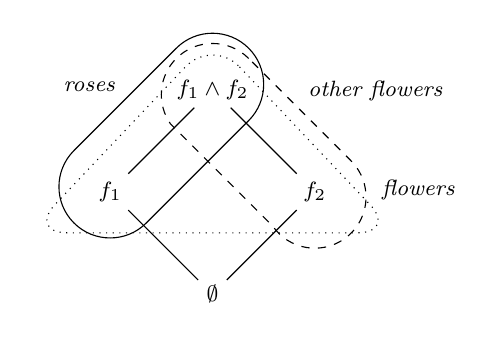
\begin{tikzpicture}[scale=1.3]
% \draw[step=0.5cm,gray,very thin] (-3.5,-3.5) grid (3.5,3.5);
\footnotesize
\node (f12) at (0,1)  {$f_1 \wedge f_2$};
\node (f1) at (-1,0) {$f_1$};
\node (f2) at (1,0) {$f_2$};
\node (neither) at (0,-1) {$\emptyset$};
\draw (f12)--(f1);
\draw (f12)--(f2);
\draw (f1)--(neither);
\draw (f2)--(neither);

%% roses
\draw (0,1) ++(0,0.05) +(-45:0.5) arc(-45:135:0.5) -- node [auto,swap] {\emph{roses}} ++(-1,-1) arc (135:315:0.5) --
++(1,1);

%% other flowers
\draw[dashed] (0,1) ++(0,-0.05) +(45:0.5) arc(45:215:0.5) -- ++(1,-1) arc (215:405:0.5) --
node [auto,swap] {\emph{other flowers}} ++(-1,1);

%% flowers
\draw[rounded corners=5mm,dotted] (0,1.5) -- node [auto, very
near end] {\emph{flowers}}   (1.8,-0.4) -- (-1.8,-0.4) -- cycle;
  
\end{tikzpicture}
\end{center}
\vspace{-0.8cm}

\caption{The domain of possible flower types, with $f_1$ the ``rose'' type and $f_2$ the non-rose flower type}
  \label{fig:1}
\end{wrapfigure}


In the first model, we rely on the technique of \emph{lexical
  uncertainty} introduced by \citet{bergen-goodman-levy:2012}.  This
technique makes the division of pragmatic labor possible by
introducing explicit reasoning over different possible mappings
between forms and pragmatically refined meanings, allowing the
efficiency of the pairing of low-cost forms with high
prior-probability meanings to be identified and subsequently
to be strengthened through recursive inference.  Fully unconstrained lexical
uncertainty, in which the meanings different utterances can be refined
in arbitrarily different ways, fails to introduce the proper bias to
consistently yield the desired strengthening of \emph{roses and flowers} to
mean \emph{roses and other flowers}.  However, we introduce
\emph{compositional} lexical uncertainty, in which simple NP
expressions (\emph{roses}, \emph{flowers}, \emph{other flowers}) can
be refined arbitrarily but complex expressions (\emph{roses and
  flowers}, \emph{roses and other flowers}) are constrained to mean
the composition of the refined meanings of their constituent parts.
Compositional lexical uncertainty does introduce a bias toward the
desired strengthening: once utterance costs are taken into account
(assuming that adding the word \emph{other} incurs some degree of
cost). 

In the second model, we relax the requirement that the literal
meanings that serve as the starting point for pragmatic inference be
categorical, truth-conditional filters on possible states of the world; rather, we allow
them to be probability distributions over these states (distinct from
the prior on world states derived from the language user's
context-specific world knowledge).  The probability distribution
associated with a coordinate NP \emph{$\alpha$ and $\beta$} is the
marginal distribution over the set of possible outcomes of the
conjuncts, which are combined by the meet operation on the lattice of
Figure~\ref{fig:1}:
%
    \begin{align*}
      P(m|\alpha\ \text{\emph{and}}\ \beta) = \sum_{m_1,m_2:m_1 \wedge m_2 = m} P(m_1|\alpha) P(m_2|\beta)
    \end{align*}
%
    This model introduces an asymmetry between the literal
    meanings of \emph{roses} and \emph{roses and flowers}, with the
    latter more strongly skewed towards the presence of more flower
    types than just roses. Recursive pragmatic inference then gives us
    the desired strengthening of \emph{roses and flowers} under a
    range of utterance cost specifications.






\def\thebibliography#1{\section*{References}
  \small
   \list
   {[\arabic{enumi}]}{\leftmargin \parindent
     \itemindent -\parindent
     \itemsep 0ex plus 1pt
     \parsep 0.1ex plus 1pt minus 1pt
     \usecounter{enumi}}
     \def\newblock{\hskip .11em plus .33em minus .07em}
     \sloppy\clubpenalty4000\widowpenalty4000
     \sfcode`\.=1000\relax}

%\bibliography{rpl-journals-long,rpl}
\bibliography{refs}
\end{document}

%%% Local Variables: 
%%% mode: latex
%%% TeX-master: t
%%% End: 
